%% Journal of Open Research Software Latex template -- Created By Stephen Bonner and John Brennan, Durham Universtiy, UK.

\documentclass{jors}

%% Set the header information
\pagestyle{fancy}
\definecolor{mygray}{gray}{0.6}
\renewcommand\headrule{}
\rhead{\footnotesize 3}
\rhead{\textcolor{gray}{UP JORS software Latex paper template version 0.1}}
\usepackage{graphicx}
\usepackage{amssymb}
\begin{document}

{\bf Software paper for submission to the Journal of Open Research Software} \\

To complete this template, please replace the blue text with your own. The paper has three main sections: (1) Overview; (2) Availability; (3) Reuse potential. \\

Please submit the completed paper to: editor.jors@ubiquitypress.com

\rule{\textwidth}{1pt}

\section*{(1) Overview}

\vspace{0.5cm}

\section*{Title}

Java Unit N-Simplex Evenly Spaced Points Generator
\section*{Paper Authors}

Giulioni, Gianfranco

\section*{Paper Author Roles and Affiliations}
Associate professor of Economics,\\ Department of Philosophical, Pedagogical and  
Economic-Quantitative Sciences,\\ University ``G. D'Annunzio'' of Chieti-Pescara,\\ 
Viale Pindaro 42 - 65127 - Pescara - ITALY

\section*{Abstract}

In a number of quantitative applications, a set of non-negative variables summing to a constant value is involved. 
A software able to generate evenly spaced points on the regular simplex (that is $N$-tuples summing to one) has been realized and it is freely available to anybody who might be interested.

\section*{Keywords}

simplex; evenly spaced points; compositional data.

\section*{Introduction}

\textcolor{blue}{An overview of the software, how it was produced, and the research for which it has been used, including references to relevant research articles. A short comparison with software which implements similar functionality should be included in this section. }

Writing a code returning a set of $N$ numbers summing to a constant is not a difficult task. The ``natural'' way to achieve the goal is to implement $N-1$ nested for cycles. However, this solution becomes inconvenient when one has to change $N$ continuously because it implies code revision. Finding a solution to change the ``dimension'' $N$ without modifying the code is not straightforward. 

A second thorny issue is to generate a grid of points on a $N$-Simplex. The main effort in performing this task is to avoid $N$-tuples duplication.

The software presented in this document provides a solution to the two problems highlighted above using object oriented programming.     

The initial motivation to develop the utility is the attempt to model agents' adaptive decision making in agent based models. More precisely, the idea was to make artificial agents able to forecast the value of a relevant variable by means of a moving arithmetic average of its past values. The weights of the arithmetic average are points on the simplex. The heuristics that characterizes adaptive behavior \cite{gigerenzeretal11} could be based on particularly easy to compute weights combinations called focal points \cite{schelling60}. Focal points are thus evenly spaced points on the simplex. In this setting, Agents have to choose which focal points to use in the next forecast. To this aim, they evaluate for each focal point the accuracy of prediction they would achieve by using the considered focal point in the past. The best performing focal point is then used to produce the next forecast. 
This mechanism is used in \cite{icaart12} in a model where firms forecast the level of demand in order to make the production. 

The application was build in order to supply the set of focal points to the artificial agents of the model.

Because a search on the Internet revealed that a user friendly software whose output complies with the above described need, I decided to realize it and to make it available to anybody that could find it useful. Hereafter, I briefly present the program functioning.

The application writes an ASCII file whose lines contain the coordinates of evenly spaced points on the unit $N$-simplex.  
It can function in GUI or in Batch mode.

The GUI opens running the Simplex without argument: \verb+java Simplex+.
Here is the application window and an example of the output file.

\vspace{1cm}

\begin{minipage}{0.5\textwidth}
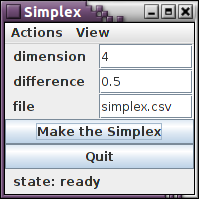
\includegraphics[scale=1]{fig1.png}
\end{minipage}
\hspace{1cm}
\begin{minipage}{0.4\textwidth}
output file 

\begin{verbatim}
0.0;0.0;0.0;1.0
0.0;0.0;0.5;0.5
0.0;0.0;1.0;0.0
0.0;0.5;0.0;0.5
0.0;0.5;0.5;0.0
0.0;1.0;0.0;0.0
0.5;0.0;0.0;0.5
0.5;0.0;0.5;0.0
0.5;0.5;0.0;0.0
1.0;0.0;0.0;0.0
\end{verbatim}
\end{minipage}

\vspace{1cm}

The three entries in the GUI are: 
\begin{itemize}
\item the dimension (denoted in this document with $N$);
\item the difference (denoted in this document with $d$);
\item and the output file name.
\end{itemize}

The program functions properly if $\frac{1}{d}$ is a positive integer ($\frac{1}{d} \in \mathbb{N}_1:=\{1,2,3,\dots \}$.
Under this condition, the output file (named according to the string found in the third text entry box) is created. Each row of the output file is a point on the simplex, that is a $N$-tuple $\{x_1,x_2,...,x_N\}$ such that
\[
\sum_{i=1}^N x_i=1
\]
and each $x_i \in \{0,d,2d,...,1\}$.

If $1/d  \notin \mathbb{N}_1$, a frame inviting you to enter a new value of $d$ appears.

%\vspace{1cm}
%\centerline{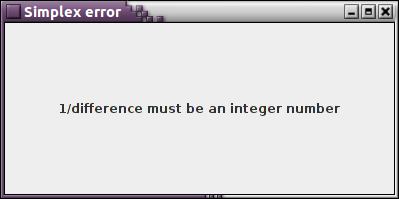
\includegraphics[scale=0.6]{fig2.png}} 


To run the program in batch mode, the three entries listed above must be supplied as arguments in the command line:\\
\verb+java Simplex <N> <d> <filename>+

The output file can be loaded by a data handling program. 
An easy example is the visualization, rescaling and shifting of points on the $\mathbb{R}^3$ unit simplex.
Figure \ref{fig:ternary}, for example reports a ternary plot of the output file.

\begin{figure}[ht]
	\centering
	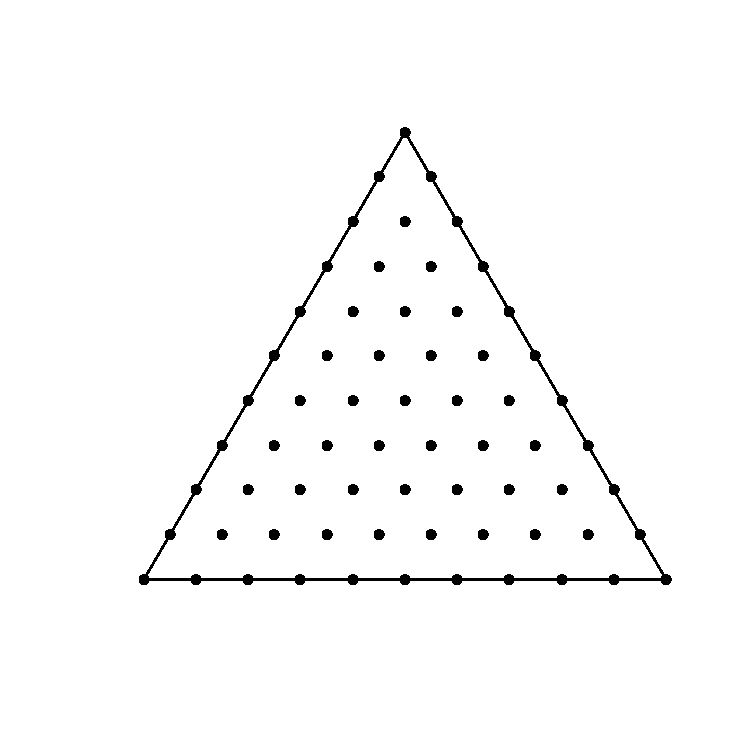
\includegraphics[scale=0.5]{fig1.pdf}
	\caption{ternary plot of the data points generated by the program with dimension $N=3$ and $d = 0.1$}
	\label{fig:ternary}
\end{figure}





\section*{Implementation and architecture}

\textcolor{blue}{How the software was implemented, with details of the architecture where relevant. Use of relevant diagrams is appropriate. Please also describe any variants and associated implementation differences.}

The architecture of this software does not present peculiarities: 
it is a Java application composed of four classes: 
\verb+Simplex+ (that contains the main), \verb+GuiBuilder+, \verb+MainWindow+, \verb+Dim+.

The code design is based on a ``cascade'' mechanism.
The core class is \verb+Dim+. Its constructor takes an integer (the identification number of its antecedent dimension) as an argument. When the constructor is executed, the \verb+Dim+ instance sets its dimension identification number as that received as an argument increased by one. It then checks if it is the last dimension, and if it is not, it creates the successive dimension as its own variable. This design allows dimension 1 to communicate with dimension 2 that can in turn communicate with dimension 3 and so on. All instances of \verb+Dim+ required by the GUI or command line dimension entry are thus created by the following line of code:\\
\verb+Dim dimension=new Dim(0);+

Once the $N$ dimensions have been created, an array of $N$ decimals is created and all its elements are set to zero.  

The \verb+iterPrint(BigDecimal[] vect)+ method allows each \verb+Dim+ instance to work on the corresponding element of the decimals vector. In particular, it computes the sum of the previous elements, say $S$, in the received vector and starts a for cycle which sets its decimal, say $s$, until $S+s$ equals 1. Of course $s \in \{0,d, 2d, \ldots\}$.   

Finally, the last dimension append the updated vector to the output file while the other dimensions call the \verb+iterPrint+ method of its successor with the updated vector as argument.

Thus, the line of code\\ \verb+dimension.iterPrint(<array of zeros>);+\\ triggers the cascade that writes the output file.




\section*{Quality control}

\textcolor{blue}{Detail the level of testing that has been carried out on the code (e.g. unit, functional, load etc.), and in which environments. If not already included in the software documentation, provide details of how a user could quickly understand if the software is working (e.g. providing examples of running the software with sample input and output data). }

Quality control for this software consists in checking that all the points are generated without duplication. Checking this is not difficult in those cases in which the number of points ($\#P(N,d)$) can be computed.

For $N=2$ for example we have
\[
	\#P(2,d)=\frac{1}{d}+1
\]
while, using the ternary plot, it is possible to show that for $N=3$ we have
\[
	\#P(3,d)=\frac{1}{2}\left[\left(\#P(2,d)\right)^2+\#P(2,d)\right].
\]

Another case in which the number of points can be computed is setting $d=0.5$ and changing $N$. In this case we have:
\[
	\#P(N,0.5)=\frac{1}{2}(N^2+N)
\]

The check consists in verifying that the number of lines in the output file is equal to $\#P(N,d)$. 


\section*{(2) Availability}
\vspace{0.5cm}
\section*{Operating system}
Platform independent.

\section*{Programming language}
Java $>$ 1.6

\section*{Additional system requirements}
None.

\section*{Dependencies}
None.

\section*{List of contributors}
No additional contributors.

\section*{Software location:}

{\bf Archive} Institutional repository 

\begin{description}[noitemsep,topsep=0pt]
	\item[Name:] simplex-master.zip
	\item[Persistent identifier:] http://erre.unich.it/giulioni/
	\item[Licence:] GPL 3.0
	\item[Publisher:]  Gianfranco Giulioni
	\item[Version published:] 1.1
	\item[Date published:] 02/09/2016
\end{description}


{\bf Code repository} GitHub

\begin{description}[noitemsep,topsep=0pt]
	\item[Name:] simplex
	\item[Persistent identifier:] https://github.com/ggiulion/simplex
	\item[Licence:] GPL 3.0
	\item[Publisher:]  Gianfranco Giulioni
	\item[Date published:] 02/09/2016
\end{description}



\section*{Language}
English.

\section*{(3) Reuse potential}

\textcolor{blue}{Please describe in as much detail as possible the ways in which the software could be reused by other researchers both within and outside of your field. This should include the use cases for the software, and also details of how the software might be modified or extended (including how contributors should contact you) if appropriate. Also you must include details of what support mechanisms are in place for this software (even if there is no support).}

The software is potentially useful in dealing with compositional data \cite{coda15}. In financial economics, for example, households are interested in determining the allocation of their wealth. Portfolio theory provides a framework to determine the shares of wealth to be allocated among the available financial assets. Therefore, the theory deals with compositional data and its outcome is a point on the unit $N$-simplex. 
Briefly, the givens of the problem are a vector of expected values and the correlation matrix of the financial assets revenues. Using these data, the first step is to build the set of all possible combinations revenue-risk that can be realized by building portfolios composed of the existing financial assets. The software can be used to have an overview of this set being each portfolio a point of the simplex. 
As an example, figure \ref{fig:portfolios} reports the set we are talking about using the output of the software with $N=3$, $d=0.01$ and the expected values and covariance matrix taken from \cite{zivot2008}. 
The ``efficient frontier'' is also reported as the thick solid black line.  

\begin{figure}[ht]
	\centering
	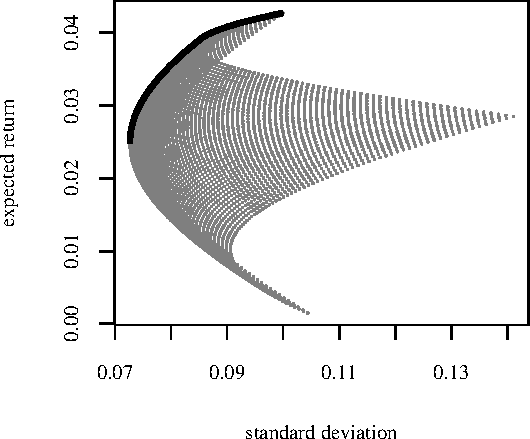
\includegraphics[scale=1.0]{set-0.pdf}
	\caption{portfolio theory: visualization of the possibility set and the efficient frontier}
	\label{fig:portfolios}
\end{figure}


Another possible application is to improve agents' adaptive decision making in agent-based computational economic models. 
We mentioned above that this aim motivated the development of the program.  
However, the set of focal points considered for example in \cite{icaart12} is static: it is generated by the Simplex program and then supplied to the agents during their initialization. Therefore, the set of focal points does not change over time. A possible improvement is to make the set of focal points dynamic by allowing the adaptive agents to change the number of terms to be considered in the moving average on the fly. In this case, when needed, the command line version of the utility presented in this paper could be called from within the agent based model to generate the new set of focal points.

A third possible use is that of random sampling from the unit simplex. \cite{sampling04} shows that it is not an easy task. In some cases, uniformly drawing a line from the output file could be a solution. 

It is very difficult to figure out the potential applications of a tool in unfamiliar fields of studies. However, compositional data widespread the real world and are thus object of study in several disciplines. The present software was build and is released with the awareness that it will bring at most a marginal contribution to those who deal with compositional data. However, we think that in sciences, it is anyway worthwhile to have small contributions because they might help in achieving more important findings. Finally, I invite people that are encountering problems in using the software or those who intend to develop it to contact me for having support.  

\section*{Acknowledgements}
None.

\section*{Funding statement}
Not funded.

\section*{Competing interests}
The author declare that he has no competing interests.



  \bibliographystyle{elsarticle-num} 
  \bibliography{osp}

%\section*{References}

%\textcolor{blue}{Please enter references in the Harvard style and include a DOI where available, citing them in the text with a number in square brackets, e.g. \\ }

%\textcolor{blue}{[1] Piwowar, H A 2011 Who Shares? Who Doesn't? Factors Associated with Openly Archiving Raw Research Data. PLoS ONE 6(7): e18657. DOI: \\ http://dx.doi.org/10.1371/journal.pone.0018657.}

\vspace{2cm}

\rule{\textwidth}{1pt}

{ \bf Copyright Notice} \\
Authors who publish with this journal agree to the following terms: \\

Authors retain copyright and grant the journal right of first publication with the work simultaneously licensed under a  \href{http://creativecommons.org/licenses/by/3.0/}{Creative Commons Attribution License} that allows others to share the work with an acknowledgement of the work's authorship and initial publication in this journal. \\

Authors are able to enter into separate, additional contractual arrangements for the non-exclusive distribution of the journal's published version of the work (e.g., post it to an institutional repository or publish it in a book), with an acknowledgement of its initial publication in this journal. \\

By submitting this paper you agree to the terms of this Copyright Notice, which will apply to this submission if and when it is published by this journal.


\end{document}
